\chapter{Convection naturelle dans et proche du noyau thermoacoustique}

Lors des expériences réalisées lors de la caractérisation du réfrigérateur TACOT, il a été montré que le gradient axial de température dans le noyau thermoacoustique n'est pas linéaire, et que les températures ne sont pas homogènes le long de la direction transverse du noyau \textcolor{red}{figure ?}\cite{ramadan_design_2021}. Cet écart au comportement attendu , c'est-à-dire un gradient linéaire entre températures froides et ambiant et une température uniforme sur la section du noyau thermoacoustique, implique la présence d'un écoulement moyen non nul dans le régénérateur. Parmi les hypothèses formulées, 

\section{Dispositif expérimental}

Pour étudier l'influence de la convection naturelle sur la distribution de température au sein du noyau thermoacoustique, le dispositif expérimental créé à l'origine du projet est modifié. Entre les deux palans visibles sur la figure~\ref{fig:TACOTSuspendu_Palans} (en gris), initialement présents pour régler l'inclinaison de la pompe à chaleur par rapport à l'axe horizontal, est placé un troisième (en bleu) pour ajouter une direction de rotation autour de l'axe de symétrie. Celui-ci

\begin{figure}[!ht]
    \centering
	\begin{subfigure}{.47\textwidth}
		\centering
		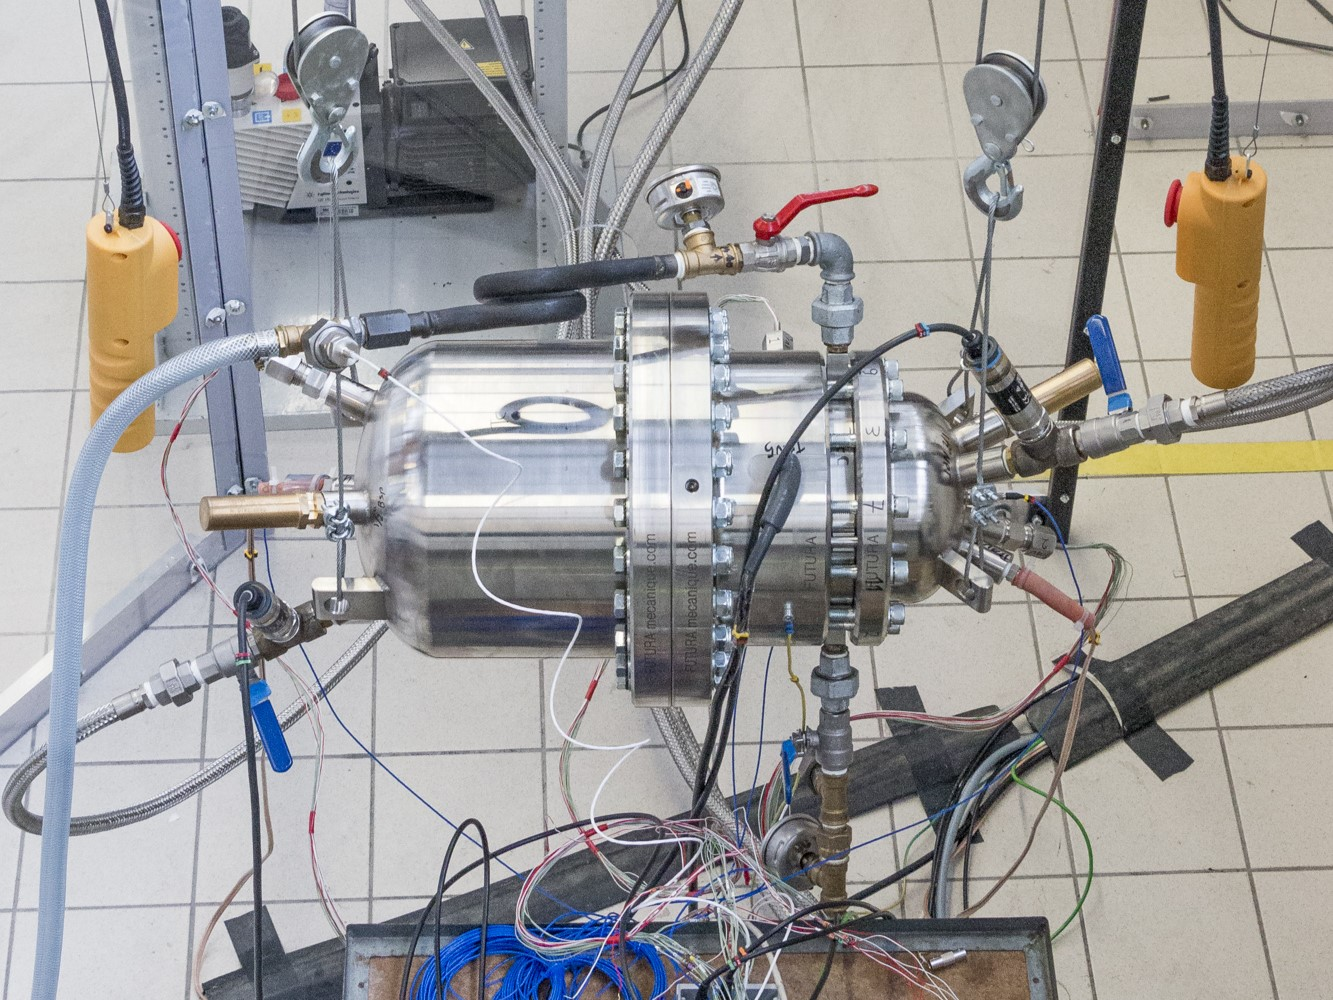
\includegraphics[width=\textwidth]{../fig/fig_SystemeAccroche/Machine_horizBetter_cropped.jpg}
		\caption{}
		\label{fig:TACOTSuspendu_Frigo}
	\end{subfigure}		
	\begin{subfigure}{.47\textwidth}
		\centering
		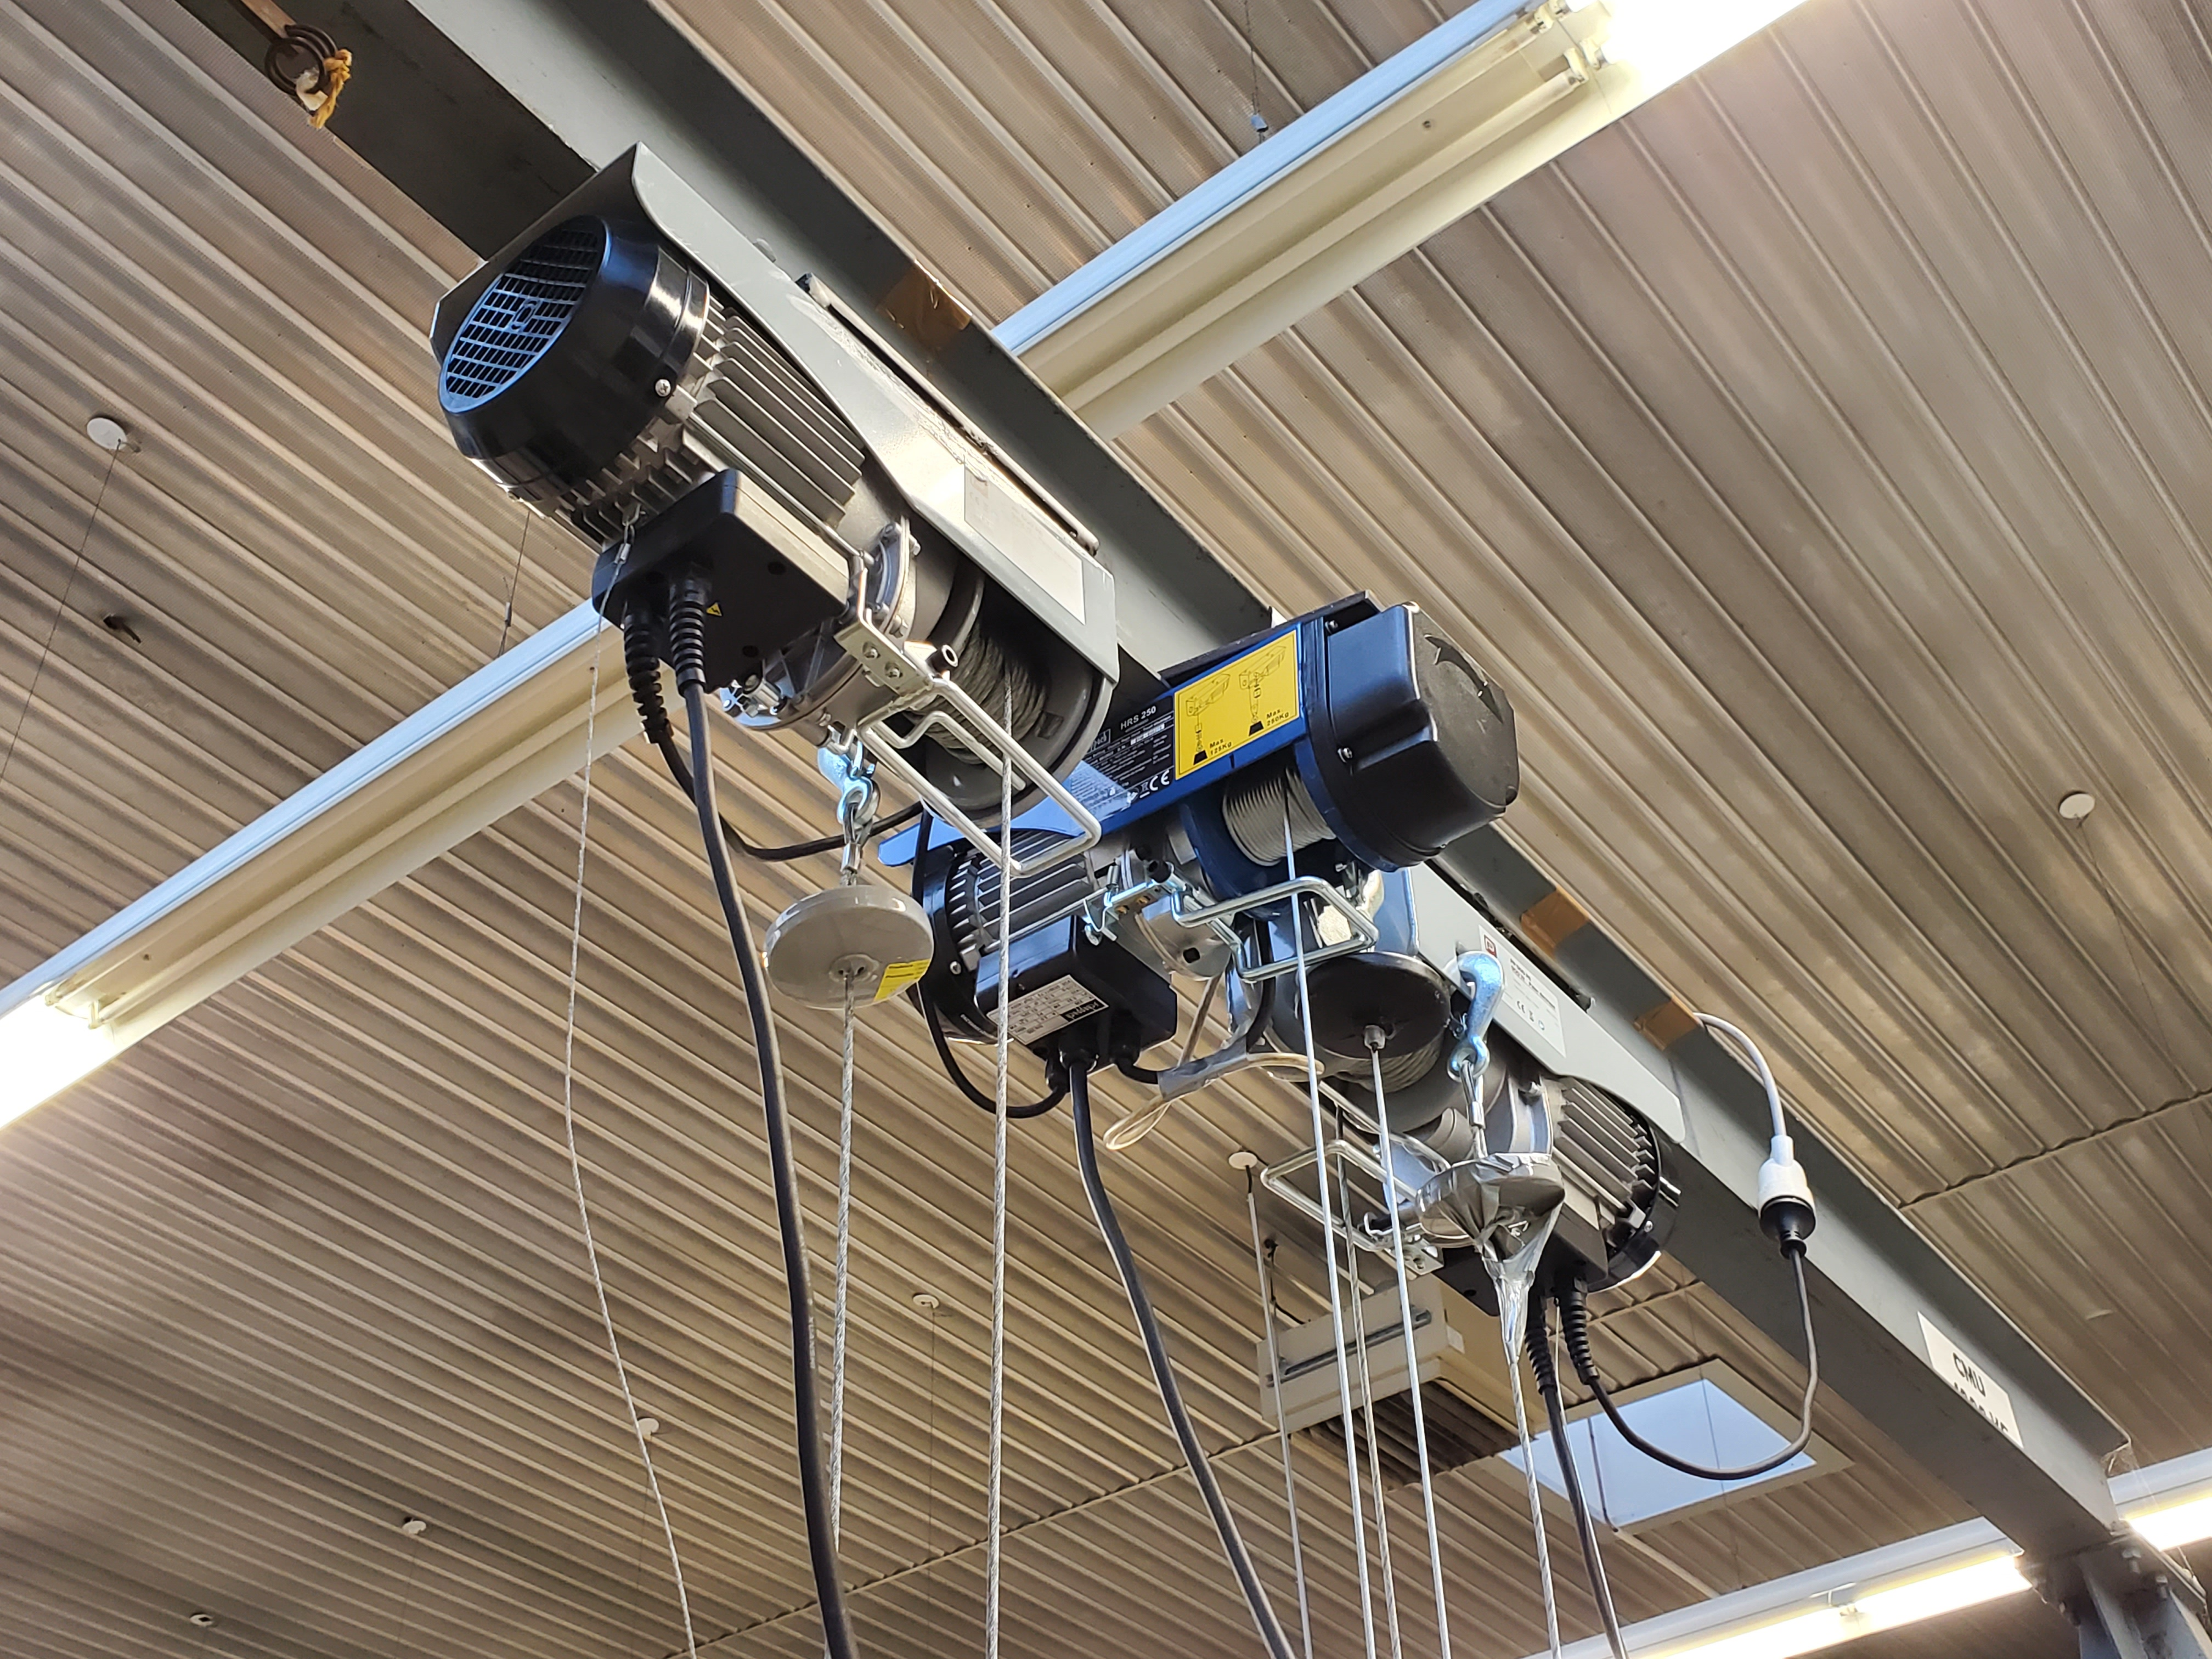
\includegraphics[width=\textwidth]{../fig/fig_SystemeAccroche/Palans.jpg}
		\caption{}
		\label{fig:TACOTSuspendu_Palans}
	\end{subfigure}	    
    \caption{Photographies \subref{fig:TACOTSuspendu_Frigo} du refrigérateur accroché et \subref{fig:TACOTSuspendu_Palans} des palans formant le système de suspension.}
    \label{fig:TACOTSuspendu}
\end{figure}

\subsection{Définition des orientations}

Les orientations choisies au moyen des palans sont décrites par deux angles. Le premier, noté $\theta_v$, désigne l'inclinaison par rapport à l'horizontal et le second, noté $\theta_h$, la rotation autour de l'axe de symétrie du réfrigérateur. Les configurations d'intérêt sont présentées sur la figure~\ref{fig:OrientationCore}, et correspondent à des \textcolor{red}{cas d'études}.

\begin{figure}[!ht]
    \centering
    \external{OrientationCore}
%    \externalremake
    \begin{tikzpicture}
%    \def\lenreg{2};
%    \def\diam{3};
    \def\spy{2};
    \def\xdist{8cm};
    \def\ydist{-7cm};
%    \def\persp{20};
%    
%    \def\LX{1};
%    \def\LY{2};
%    \def\CoreX{1.5};
%    \def\CoreY{.9*\LY};
%    

	\def\L{2};
	\def\R{6};
	\def\HX{.25};
	\def\decalage{\R/2-\L/2};
    
%	Islam's idea
	\begin{scope}
%		\begin{tikzpicture}[scale=2/3]

%    \def\lenreg{2};
%    \def\diam{3};
    \def\spy{2};
    \def\xdist{8cm};
    \def\ydist{-7cm};
%    \def\persp{20};
%    
%    \def\LX{1};
%    \def\LY{2};
%    \def\CoreX{1.5};
%    \def\CoreY{.9*\LY};
%    

	\def\L{2.1};
	\def\R{5};
	\def\HX{.25};
	\def\decalage{\R/2-\L/2};
	
		\draw(6.5,\R/2) node{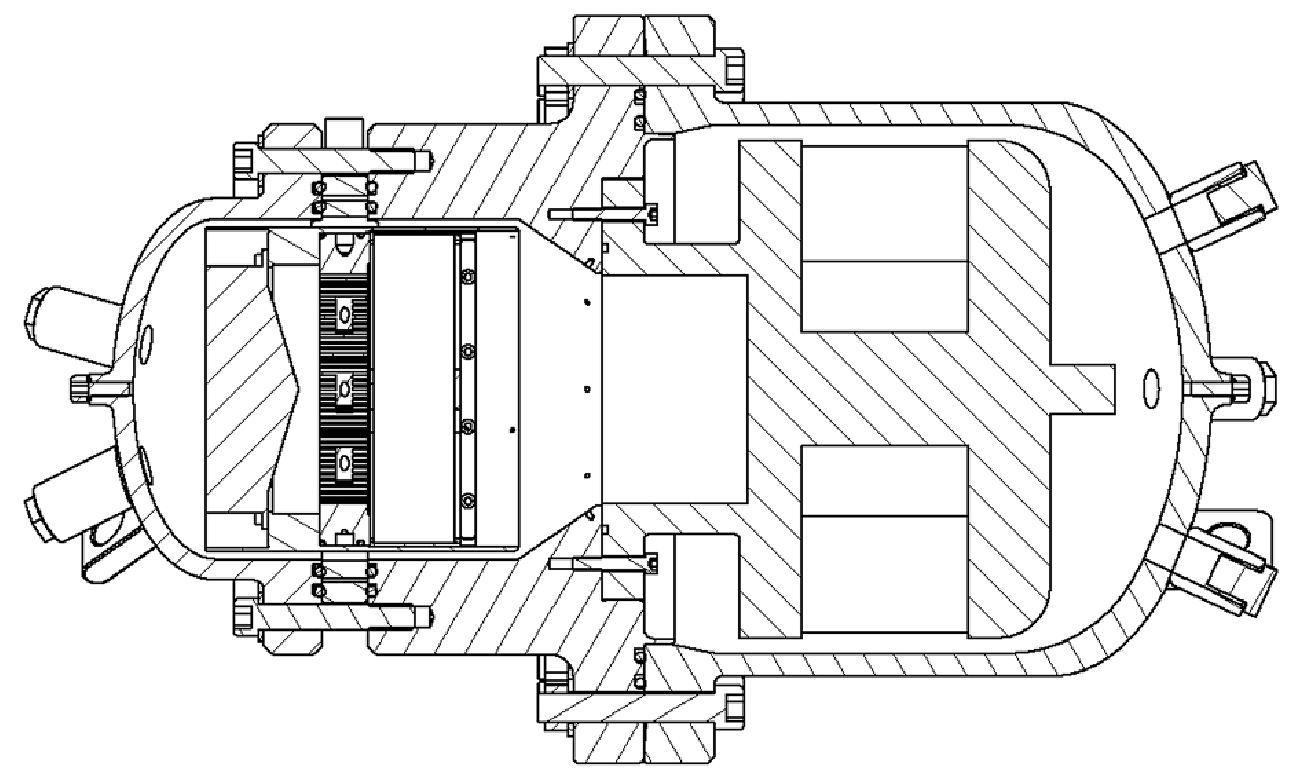
\includegraphics[width=.8\textwidth]{../fig/fig_OrientationCore/tex/TACOT.png}};
			
		\fill[right color=blue!25,left color=red!25, draw=black] (\decalage,0) rectangle ++(\L,\R);
		\draw[fill=red!25] (\decalage,0) rectangle ++(-\HX,\R);
		\draw[fill=blue!25] (\decalage+\L,0) rectangle ++(\HX,\R);

		\foreach \z [evaluate=\z] in {0,...,4}{
			\foreach \r [evaluate=\r as \num using int(\r+1 + 3*\z)] in {0,...,2}{
				\draw ({\decalage+.5+\L-\z*(1+\L)/4},{-(\R-.4)/2*\r+\R-.2}) node[minimum size=10pt,draw,circle,fill=white,opacity=.7,text opacity=1]{} node(n\z\r){\scriptsize \num};
}}

%		\draw (n01.east) node [right]{0 $\rightarrow$ \begin{tabular}{l}Source\\acoustique\\principale\end{tabular}};
		\draw ($(n01)+(1.5,0)$) node[minimum size=10pt,draw,circle,fill=white,opacity=.7,text opacity=1]{} node(RIX) {\scriptsize 0};% node[anchor=west]{\begin{tabular}{rl}
%		& Source\\
%		$\rightarrow$ & acoustique\\
%		& principale
%		\end{tabular}};
		\draw (n30.north west) node [above, fill=white, fill opacity=.7, text opacity=1]{Ambiant};
		\draw (n10.north east) node [above, fill=white, fill opacity=.7, text opacity=1]{Froid};
\end{tikzpicture}
		\fill[right color=blue!25,left color=red!25, draw=black] (\decalage,0) rectangle ++(\L,\R);
		\draw[fill=red!25] (\decalage,0) rectangle ++(-\HX,\R);
		\draw[fill=blue!25] (\decalage+\L,0) rectangle ++(\HX,\R);

		\foreach \z [evaluate=\z] in {0,...,4}{
			\foreach \r [evaluate=\r as \num using int(\r+1 + 3*\z)] in {0,...,2}{
				\draw ({\decalage+.5+\L-\z*(1+\L)/4},{-(\R-.4)/2*\r+\R-.2}) node(n\z\r){\num};
}}

		\draw (n01.east) node [right]{$\rightarrow$ \begin{tabular}{l}Source\\acoustique\\principale\end{tabular}};
		\draw (n30.north west) node [above]{AHX};
		\draw (n10.north east) node [above]{CHX};

		\draw (0,\R+\spy) node [anchor=west]{\textbf{(a)} \texttt{H1}};

	\end{scope}
	
	
	
	\begin{scope}[xshift=\xdist-1cm,yshift=2cm]
		\begin{scope}[xslant=1,yscale=.5]
%		\begin{tikzpicture}[scale=2/3]

%    \def\lenreg{2};
%    \def\diam{3};
    \def\spy{2};
    \def\xdist{8cm};
    \def\ydist{-7cm};
%    \def\persp{20};
%    
%    \def\LX{1};
%    \def\LY{2};
%    \def\CoreX{1.5};
%    \def\CoreY{.9*\LY};
%    

	\def\L{1};
	\def\R{5};
	\def\HX{.25};
	\def\decalage{\R/2-\L/2};
	
%	\draw[opacity=0] (\decalage,0) rectangle ++(-\HX,\R); %%% Pour l'alignement vertical
%\draw{[white](\L/2,0) -- ++(0,\R);
	
	\begin{scope}[yslant=-1]
		\begin{scope}[xslant=.71]%, rotate=90, xscale=1]
		\node at (\decalage-\HX,0) (NewO) {};
%		\draw[->, very thick] (NewO.center) -- ++(0,1.2*\R);
%		\draw[->, very thick] (NewO.center) -- ++(1.2*\R,0);
		
		\fill[shading=axis,right color=MatlabBlue,left color=MatlabOrange, shading angle=22.5, draw=black] (\decalage,0) rectangle ++(\L,\R*1.4);
		\draw[fill=MatlabOrange] (\decalage,0) rectangle ++(-\HX,\R*1.4);
		\draw[fill=MatlabBlue] (\decalage+\L,0) rectangle ++(\HX,\R*1.4);

		\foreach \z [evaluate=\z] in {0,...,4}{
			\foreach \r [evaluate=\r as \num using int(\r+1 + 3*\z)] in {0,...,2}{
				\draw ({\decalage+.5+\L-\z*(1+\L)/4},{-(\R*1.4-.4)/2*\r+\R*1.4-.2}) node[minimum size=10pt,draw,circle,fill=white,opacity=.7,text opacity=1]{} node(n\z\r){\scriptsize \num};
}}

%		\draw (n01.east) node [right]{$\rightarrow$ \begin{tabular}{l}Source\\acoustique\\principale\end{tabular}};
		\draw ($(n01)+(.75,0)$) node[minimum size=10pt,draw,circle,fill=white,opacity=.7,text opacity=1]{} node {\scriptsize 0};% node[anchor=west]{\begin{tabular}{rl}
%		& Src\\
%		$\rightarrow$ & ac\\
%		& princ
%		\end{tabular}};
%		\draw (n30.north west) node [above right, fill=white, fill opacity=0, text opacity=1]{\textcolor{MatlabOrange}{\textbf{Ambiant}}};
%		\draw (n10.north east) node [above right, fill=white, fill opacity=0, text opacity=1]{\textcolor{MatlabBlue}{\textbf{Froid}}};
		
	\end{scope}
	\end{scope}
	\begin{pgfonlayer}{background}
		\draw[->, very thick] (NewO.center) -- ++(22.5:1.2*\R) node [above] {$\mathbf e_{y,0}$};
		\draw[->, very thick] (NewO.center) -- ++(90:1.2*\R) node [left] {$\mathbf e_{z,0}$};
		\draw[->, very thick] (NewO.center) -- ++(-45:1.2*\R) node [right] {$\mathbf e_{x,0}$};
  	\end{pgfonlayer}
\end{tikzpicture}
		\fill[right color=blue!25,left color=red!25, draw=black] (\decalage,0) rectangle ++(\L,\R);
		\draw[fill=red!25] (\decalage,0) rectangle ++(-\HX,\R);
		\draw[fill=blue!25] (\decalage+\L,0) rectangle ++(\HX,\R);

		\foreach \z [evaluate=\z] in {0,...,4}{
			\foreach \r [evaluate=\r as \num using int(\r+1 + 3*\z)] in {0,...,2}{
				\draw ({\decalage+.5+\L-\z*(1+\L)/4},{-(\R-.4)/2*\r+\R-.2}) node(n\z\r){\num};
}}

		\draw (n01.east) node [right]{$\rightarrow$ \begin{tabular}{l}Source\\acoustique\\principale\end{tabular}};
		\draw (n30.north west) node [above]{AHX};
		\draw (n10.north east) node [above]{CHX};
		\end{scope}

		\draw (1cm,\R+\spy-2cm) node [anchor=west]{\textbf{(b)} \texttt{H2}};
	\end{scope}  
	
	
	  
	\begin{scope}[yshift=\ydist]
%		%\fill[top color=red!25, bottom color=blue!25, draw=black] (0,0) rectangle ++(\R,\L);
%\draw[fill=blue!25] (0,0) rectangle ++(\R,-\HX);
%\draw[fill=red!25] (0,\L) rectangle ++(\R,\HX);
%
%\foreach \z [evaluate=\z] in {0,...,4}{
%	\foreach \r [evaluate=\r as \num using int(\r+1 + 3*\z)] in {0,...,2}{
%		\draw ({-(\R-.4)/2*\r+\R-.2},{\z*(1+\L)/4-.5}) node(n\z\r){\num};
%}}
%
%\draw (n40.south east) node [right]{AHX};
%\draw (n00.north east) node[right]{CHX};
%\draw (n01.south) node [below]{\shortstack{ $\downarrow$ \\Source acoustique principale}};
%
%\draw (0,\L+2*\HX+\spy) node [anchor=west]{\textbf{(c)} \texttt{V1}};

\begin{tikzpicture}[scale=2/3]

%    \def\lenreg{2};
%    \def\diam{3};
    \def\spy{2};
    \def\xdist{8cm};
    \def\ydist{-7cm};
%    \def\persp{20};
%    
%    \def\LX{1};
%    \def\LY{2};
%    \def\CoreX{1.5};
%    \def\CoreY{.9*\LY};
%    

	\def\L{2};
	\def\R{5};
	\def\HX{.35};
	\def\decalage{\R/2-\L/2};
	
	\begin{scope}[yslant=tan(22.5)]	
		
		\node at (0,-\HX) (NewO) {};
	
		\fill[shading=axis,right color=MatlabBlue,left color=MatlabOrange, shading angle=22.5, draw=black] (0,0) rectangle ++(\R,\L);
		\draw[fill=MatlabBlue] (0,0) rectangle ++(\R,-\HX);
		\draw[fill=MatlabOrange] (0,\L) rectangle ++(\R,\HX);

		\foreach \z [evaluate=\z] in {0,...,4}{
			\foreach \r [evaluate=\r as \num using int(\r+1 + 3*\z)] in {0,...,2}{
				\draw ({-(\R-.4)/2*\r+\R-.2},{\z*(1+\L)/4-.5}) node[minimum size=10pt,draw,circle,fill=white,opacity=.7,text opacity=1]{} node(n\z\r){\scriptsize \num};
}}

%		\draw (n40.south east) node [right, fill=white, fill opacity=0, text opacity=1]{\textcolor{MatlabOrange}{\textbf{Ambiant}}};
%		\draw (n00.north east) node[right, fill=white, fill opacity=0, text opacity=1]{\textcolor{MatlabBlue}{\textbf{Froid}}};
		\draw ($(n01.south)+(0,-1.1)$) node[minimum size=10pt,draw,circle,fill=white,opacity=.7,text opacity=1]{} node (RIX){\scriptsize 0};% node[anchor=north]{\begin{tabular}{c}
%		$\downarrow$\\
%		Source acoustique principale
%		\end{tabular}};

	\end{scope}
	\begin{pgfonlayer}{background}
		\draw[->, very thick] (NewO.center) -- ++(22.5:1.2*\R) node [above] {$\mathbf e_{y,0}$};
		\draw[->, very thick] (NewO.center) -- ++(90:1.2*\R) node [left] {$\mathbf e_{z,0}$};
		\draw[->, very thick] (NewO.center) -- ++(-45:1.2*\R) node [right] {$\mathbf e_{x,0}$};
  	\end{pgfonlayer}		
\end{tikzpicture}		

		\fill[top color=red!25, bottom color=blue!25, draw=black] (0,0) rectangle ++(\R,\L);
		\draw[fill=blue!25] (0,0) rectangle ++(\R,-\HX);
		\draw[fill=red!25] (0,\L) rectangle ++(\R,\HX);

		\foreach \z [evaluate=\z] in {0,...,4}{
			\foreach \r [evaluate=\r as \num using int(\r+1 + 3*\z)] in {0,...,2}{
				\draw ({-(\R-.4)/2*\r+\R-.2},{\z*(1+\L)/4-.5}) node(n\z\r){\num};
}}

		\draw (n40.south east) node [right]{AHX};
		\draw (n00.north east) node[right]{CHX};
		\draw (n01.south) node [below]{\shortstack{ $\downarrow$ \\Source acoustique principale}};

		\draw (0,\L+2*\HX+\spy) node [anchor=west]{\textbf{(c)} \texttt{V1}};
	\end{scope} 
	
	
	
	   
	\begin{scope}[xshift=\xdist,yshift=\ydist]
%		%\fill[top color=blue!25, bottom color=red!25, draw=black] (0,0) rectangle ++(\R,\L);
%\draw[fill=red!25] (0,0) rectangle ++(\R,-\HX);
%\draw[fill=blue!25] (0,\L) rectangle ++(\R,\HX);
%
%\foreach \z [evaluate=\z] in {0,...,4}{
%	\foreach \r [evaluate=\r as \num using int(\r+1 + 3*\z)] in {0,...,2}{
%		\draw ({(\R-.4)/2*\r+.2},{-\z*(1+\L)/4+\L+.5}) node(n\z\r){\num};
%}}
%
%\draw (n01.north) node [above]{\shortstack{Source acoustique principale\\ $\uparrow$}};
%\draw (n42.north east) node [right]{AHX};
%\draw (n02.south east) node [right]{CHX};
%
%\draw (0,\L+2*\HX+\spy) node [anchor=west]{\textbf{(d)} \texttt{V2}};

\begin{tikzpicture}[scale=2/3]

%    \def\lenreg{2};
%    \def\diam{3};
    \def\spy{2};
    \def\xdist{8cm};
    \def\ydist{-7cm};
%    \def\persp{20};
%    
%    \def\LX{1};
%    \def\LY{2};
%    \def\CoreX{1.5};
%    \def\CoreY{.9*\LY};
%    

	\def\L{2.1};
	\def\R{5};
	\def\HX{.25};
	\def\decalage{\R/2-\L/2};

		\fill[top color=MatlabBlue, bottom color=MatlabOrange, draw=black] (0,0) rectangle ++(\R,\L);
		\draw[fill=MatlabOrange] (0,0) rectangle ++(\R,-\HX);
		\draw[fill=MatlabBlue] (0,\L) rectangle ++(\R,\HX);

		\foreach \z [evaluate=\z] in {0,...,4}{
			\foreach \r [evaluate=\r as \num using int(\r+1 + 3*\z)] in {0,...,2}{
				\draw ({(\R-.4)/2*\r+.2},{-\z*(1+\L)/4+\L+.5}) node[minimum size=10pt,draw,circle,fill=white,opacity=.7,text opacity=1]{} node(n\z\r){\scriptsize \num};
}}

		\draw ($(n01.north)+(0,1.1)$) node[minimum size=10pt,draw,circle,fill=white,opacity=.7,text opacity=1]{} node(RIX){\scriptsize 0};% node[anchor=south]{\begin{tabular}{c}
%		Source acoustique principale\\
%		$\uparrow$
%		\end{tabular}};
		\draw (n42.north east) node [right, fill=white, fill opacity=.7, text opacity=1]{\textcolor{MatlabOrange}{\textbf{Ambiant}}};
		\draw (n02.south east) node [right, fill=white, fill opacity=.7, text opacity=1]{\textcolor{MatlabBlue}{\textbf{Froid}}};
%		\draw (n41.south) node [below]{\textcolor{white}{\shortstack{Source acoustique principale\\ $\uparrow$}}};
		
\end{tikzpicture}	
		\fill[top color=blue!25, bottom color=red!25, draw=black] (0,0) rectangle ++(\R,\L);
		\draw[fill=red!25] (0,0) rectangle ++(\R,-\HX);
		\draw[fill=blue!25] (0,\L) rectangle ++(\R,\HX);

		\foreach \z [evaluate=\z] in {0,...,4}{
			\foreach \r [evaluate=\r as \num using int(\r+1 + 3*\z)] in {0,...,2}{
				\draw ({(\R-.4)/2*\r+.2},{-\z*(1+\L)/4+\L+.5}) node(n\z\r){\num};
}}

		\draw (n01.north) node [above]{\shortstack{Source acoustique principale\\ $\uparrow$}};
		\draw (n42.north east) node [right]{AHX};
		\draw (n02.south east) node [right]{CHX};

		\draw (0,\L+2*\HX+\spy) node [anchor=west]{\textbf{(d)} \texttt{V2}};	
	\end{scope}    
    
%	 Alternate version    
%    \draw[->] (5.5,-.5) -- ++(1,0);\draw(6,-1) node[]{Vertical 2};
%    \draw[->] (6.5,.5) -- ++(-1,0);\draw(6,1) node[]{Vertical 1};
%    \draw[->] (9,.5) -- ++(0,-1);\draw(9,1) node[]{Horizontal 1};
%    \draw (12,0) node[circle,draw]{.};\draw (12,1) node[]{Horizontal 2};
%    
%    
%    \draw[line width=.5mm] (-2.5*\LX,0) to[out=90,in=-180] (-\LX,\LY) -- ++(2*\LX,0) -- ++(.5*\LX,-2*\LY/3) -- ++(.2*\LX,0) -- ++(0,2*\LY/3);
\draw[line width=.5mm] (\LX,\LY) -- ++(\LX,0) to[out=0,in=90] (3.5*\LX,0);

\fill[left color=red,right color=blue] ({-\LX+.4*\CoreX},0) rectangle ({-\LX+.9*\CoreX},\CoreY);
\draw[line width=.5mm] (-\LX,\CoreY) -- ++(\CoreX,0);
\draw[fill=PythonBlue] (-.9*\LX,0) -- ++(0,\CoreY) to[out=-80,in=90] (-.7*\LX,0);
\draw ({-\LX+.4*\CoreX},0) -- ++(0,\CoreY);
\draw ({-\LX+.9*\CoreX},0) -- ++(0,\CoreY);

\draw[fill=PythonBlue] (1.6*\LX,0) |- ++(.3*\LX,.9*\LY/3) |- ++(\LX,.2*\LY) arc (90:0:.05) -- ++(0,-.5*\LY);
%    \begin{scope}[yscale=-1]
%        \draw[line width=.5mm] (-2.5*\LX,0) to[out=90,in=-180] (-\LX,\LY) -- ++(2*\LX,0) -- ++(.5*\LX,-2*\LY/3) -- ++(.2*\LX,0) -- ++(0,2*\LY/3);
\draw[line width=.5mm] (\LX,\LY) -- ++(\LX,0) to[out=0,in=90] (3.5*\LX,0);

\fill[left color=red,right color=blue] ({-\LX+.4*\CoreX},0) rectangle ({-\LX+.9*\CoreX},\CoreY);
\draw[line width=.5mm] (-\LX,\CoreY) -- ++(\CoreX,0);
\draw[fill=PythonBlue] (-.9*\LX,0) -- ++(0,\CoreY) to[out=-80,in=90] (-.7*\LX,0);
\draw ({-\LX+.4*\CoreX},0) -- ++(0,\CoreY);
\draw ({-\LX+.9*\CoreX},0) -- ++(0,\CoreY);

\draw[fill=PythonBlue] (1.6*\LX,0) |- ++(.3*\LX,.9*\LY/3) |- ++(\LX,.2*\LY) arc (90:0:.05) -- ++(0,-.5*\LY);
%    \end{scope}
    
    % Old version
    % %%%%%%%%%%%%%%%%%%%% V1
    % \fill[bottom color=PythonBlue, top color=PythonRed,draw=black] (-\xdist,{\ydist+\lenreg}) -- ++(0,{-\lenreg}) arc (0:-180:{\diam} and {\diam/\persp}) -- ++(0,{\lenreg}) arc (-180:0:{\diam} and {\diam/\persp}) --cycle;
    
    % \draw[fill=PythonRed] ({-\xdist-\diam},\ydist+\lenreg) ellipse ({\diam} and {\diam/\persp});
    
    % \draw ({-\xdist-\diam},\ydist-\spy) node []{\textbf{(a)} V1};
    
    
    % %%%%%%%%%%%%%%%%%%%% V2
    % \fill[bottom color=PythonRed, top color=PythonBlue,draw=black] (\xdist,{\ydist+\lenreg}) -- ++(0,{-\lenreg}) arc (-180:0:{\diam} and {\diam/\persp}) -- ++(0,{\lenreg}) arc (0:-180:{\diam} and {\diam/\persp}) --cycle;
    
    % \draw[fill=PythonBlue] ({\xdist+\diam},\ydist+\lenreg) ellipse ({\diam} and {\diam/\persp});
    
    % \draw ({\xdist+\diam},\ydist-\spy) node []{\textbf{(b)} V2};
    
    
    % %%%%%%%%%%%%%%%%%%%% H1
    % \draw ({-\xdist-\diam},-\ydist) circle (\diam);
    % \draw[dashed,very thick] ({-\xdist-\diam},{-\ydist+\diam}) -- ++(0,-2*\diam);
    
    % \draw ({-\xdist-\diam},-\ydist-\diam-\spy) node []{\textbf{(c)} H1};
    
    
    % %%%%%%%%%%%%%%%%%%%% H2
    % \draw ({\xdist+\diam},-\ydist) circle (\diam);
    % \draw[dashed,very thick] ({\xdist},{-\ydist}) -- ++(2*\diam,0);
    
    % \draw ({\xdist+\diam},-\ydist-\diam-\spy) node []{\textbf{(d)} H2};
\end{tikzpicture}
    \caption{Différentes orientations du c\oe{}ur thermoacoustique avec les positions des thermocouples et leurs numéro. Pour chaque cas, la gravité est orientée vers le bas.\textcolor{red}{Faire le lien avec $\theta_v$ et $\theta_h$ ?}}
    \label{fig:OrientationCore}
\end{figure}


\subsection{Adimensionnement des données de température}

Pour comparer les données de température relatives les unes aux autres, il est judicieux d'exprimer $T(x,r)$ dans l'intervalle $[0,1]$ en définissant la température adimensionnée $\tau(x,r)$ telle que

\begin{equation}
    \tau(x,r) = \frac{T(x,r)-T_c}{T_a - T_c}\quad,
    \label{eq:TemperatureAdimension}
\end{equation}
où $T_a$ et $T_c$ sont les températures ambiante et froide mesurées sur l'axe du noyau thermoacoustique.


\section{Protocole expérimental}

Le protocole de mesure suivi pour l'acquisition des données expérimentale comporte plusieurs parties. Tout d'abord, l'eau est mise en circulation dans l'échangeur ambiant à un débit de \qty{7}{\l\per\minute},

Les conditions expérimentales sont présentées Tab~\ref{tab:RecapCondExpe}.

\begin{table}[!ht]
\centering
	\begin{tabular}{ccccccccc}
		\hline
		$\xi_1$ [\unit{\mm}] & $\xi_2$ [\unit{\mm}] & $\varphi_{2-1}$ [\unit{\degree}] & $DR$ [\unit{\percent}] & $T_a$ [\unit{\degreeCelsius}] & $\dot Q_a$ [\unit{\W}] & $T_c$ [\unit{\degreeCelsius}] & $\dot Q_c$ [\unit{\W}] & Orientation \\\hline\hline
		\num{0} & \num{0} & -- & \num{0} & & & & & V1 \\
		\num{0} & \num{0} & -- & \num{0} & & & & & V2\\%\hline
		\num{1} & \num{.28} & \num{-60} & \num{.4} & \textbf{\num{15.1}} | \textit{\num{15.1}} & \num{1.29} & \textbf{\num{10.9}} | \textit{\num{13}} & \num{0} & V1 \\
		\num{1.1} & \num{.30} & \num{-60} & \num{.4} & \textbf{\num{15.3}} | \textit{\num{14.2}}& \num{.11} & \textbf{\num{12.3}} | \textit{\num{13.4}} & \num{0} & V2 \\
		\num{1} & \num{.28} & \num{-60} & \num{.4} & \textbf{\num{16.7}} | \textit{\num{16}}& \num{-.40} & \textbf{\num{16.2}} | \textit{\num{17}} & \num{10} & V1 \\
		\num{1.1} & \num{.32} & \num{-60} & \num{.4} &\textbf{ \num{16}} | \textit{\num{14.6}} & \num{4.47} & \textbf{\num{15.9}} | \textit{\num{16.9}} & \num{6.43} & V2 \\%\hline
		\num{4} & \num{.89} & \num{-60} & \num{1.7} & \textbf{\num{10.6}} | \textit{\num{17.3}} & \num{33.8} & \textbf{\num{-8.82}} | \textit{\num{-1.92}} & \num{0} & V1 \\
		\num{5} & \num{1.14} & \num{-60} & \num{1.7} & \textbf{\num{18.65}} | \textit{\num{16.5}} & \num{75} & \textbf{\num{-14.24}} | \textit{\num{-9.85}} & \num{0} & V2 \\
		\num{4} & \num{.87} & \num{-60} & \num{1.7} & \textbf{\num{28}} | \textit{\num{27.6}} & \num{67.54} & \textbf{\num{27.83}} | \textit{\num{30.12}}& \num{135} & V1 \\
		\num{5} & \num{1.1} & \num{-60} & \num{1.7} & \textbf{\num{31.59}} | \textit{\num{24.06}} & \num{143.94} & \textbf{\num{31.7}} | \textit{\num{36.1}} & \num{219} & V2 \\%\hline
		\num{8.3} & \num{1.63} & \num{-60} & \num{3.5} & \textbf{\num{30.12}} | \textit{\num{30.98}} & \num{175.03} & \textbf{\num{-20.47}} | \textit{\num{-14.53}} & \num{0} & V1 \\
		\num{8.4} & \num{1.68} & \num{-60} & \num{3.5} & \textbf{\num{22.33}} | \textit{\num{18.85}} & \num{217.72} & \textbf{\num{-24.53}} | \textit{\num{-16.81}} & \num{0} & V2 \\
		\num{8.3} & \num{1.56} & \num{-60} & \num{3.5} & \textbf{\num{32.58}} | \textit{\num{35.02}} & \num{240.56} &\textbf{\num{-6.03}} | \textit{\num{2.8}}  & \num{112} & V1 \\
		\num{8.3} & \num{1.66} & \num{-60} & \num{3.5} & \textbf{\num{27.28}} | \textit{\num{22.24}} & \num{254.95} & \textbf{\num{-6.6}} | \textit{\num{-1.22}} & \num{112} & V2 \\
		\num{8.4} & \num{1.56} & \num{-60} & \num{3.5} & \textbf{\num{33.51}} | \textit{\num{36.85}} & \num{264.78} & \textbf{\num{2.08}} | \textit{\num{11.77}} & \num{219} & V1 \\
		\num{8.3} & \num{1.63} & \num{-60} & \num{3.5} & \textbf{\num{30.71}} | \textit{\num{24.89}} & \num{290.28} & \textbf{\num{3.87}} | \textit{\num{11.64}} & \num{219} & V2 \\
		\num{8.3} & \num{1.54} & \num{-60} & \num{3.5} & \textbf{\num{38.5}} | \textit{\num{40.92}} & \num{303.34} & \textbf{\num{16.36}} | \textit{\num{25.87}} & \num{330} & V1 \\
		\num{8.3} & \num{1.62} & \num{-60} & \num{3.5} & \textbf{\num{36.35}} | \textit{\num{28.01}} & \num{304.32} & \textbf{\num{16.77}} | \textit{\num{24.67}} & \num{330} & V2 \\
		\num{8.3} & \num{1.54} & \num{-60} & \num{3.5} & \textbf{\num{40.59}} | \textit{\num{42.37}} & \num{298.5} & \textbf{\num{28.57}} | \textit{\num{37.68}} & \num{446} & V1 \\
		\num{8.4} & \num{1.6} & \num{-60} & \num{3.5} & \textbf{\num{35.55}} | \textit{\num{29.27}} & \num{333.64} & \textbf{\num{29.52}} | \textit{\num{39.74}} & \num{446} & V2 \\%\hline
%%		\num{0} & \num{0} & - & \num{0} & & & & & H1 \\
%%		\num{0} & \num{0} & - & \num{0} & & & & & H2 \\%\hline
%		\num{8.5} & \num{} & \num{-60} & \num{3.5} & \textbf{\num{}} | \textit{\num{}} & \num{} & \textbf{\num{}} | \textit{\num{}} & \num{0} & H1 \\
%		\num{8.5} &\num{}  & \num{-60} & \num{3.5} & \textbf{\num{}} | \textit{\num{}} & \num{} & \textbf{\num{}} | \textit{\num{}} & \num{0} & H2 \\
%		\num{8.5} & \num{} & \num{-60} & \num{3.5} & \textbf{\num{}} | \textit{\num{}} & \num{} & \textbf{\num{}} | \textit{\num{}} & \num{1212} & H1 \\
%		\num{8.5} & \num{} & \num{-60} & \num{3.5} & \textbf{\num{}} | \textit{\num{}} & \num{} & \textbf{\num{}} | \textit{\num{}} & \num{1212} & H2 \\
\hline
	\end{tabular} %\textbf{\num{}} | \textit{\num{}}
	\caption{Tableau récapitulatif des conditions expérimentales.\textcolor{red}{Pression ac  ?} Les déplacements $\xi$ sont exprimés en valeur ``crête'', les températures en \textbf{gras} sont mesurées au centre du noyau, celles en \textit{italique} sont le résultat d'une moyenne sur la section.}
	\label{tab:RecapCondExpe}
\end{table}


\section{Cellule de convection naturelle entre la source principale et le noyau thermoacoustique}

\section{Résultats}

\subsection{\'Etude des données temporelles de température}

En première approche, les données de température en fonction du temps sont tracées pour être analysées. Elles comportent des informations sur le régime transitoire, et sont assez longues pour mesurer les températures atteintes en régime établi. Leur durée permet également de vérifier la présence ou l'absence de phénomènes d'instabilités observés lors de mesures préliminaires.

\begin{figure}[!ht]
    \centering
    \external{fig_Vert2_LowRix_Acou}
    %\externalremake
    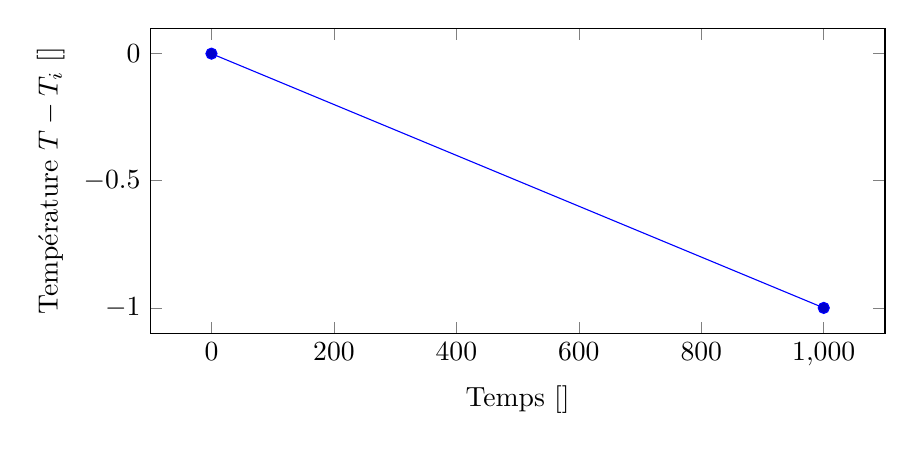
\begin{tikzpicture}
    \def\width{.9*\textwidth};
    \def\height{.5*\width};
    \def\spx{.25cm};
    \def\spy{1.25cm};
    \def\legx{.5cm};
    \def\legy{\legx};
    \def\prop{.45};
    
    \begin{axis}[name=TC,width={\width},height={\height},
    xlabel={Temps [\unit{\s}]},
    ylabel={Température $T - T_i$ [\unit{\degree}]},
%    xmin=0,xmax=75,ymin=0,ymax=.5/1000,
%    xtick={0,25,47,50,75,100},ytick={0,9.1120/100000,1.4452/10000,2.5/10000,5/10000,1/1000},
    legend style = {at={(.95,.95)},anchor = north east}
    ]
       \addplot coordinates {(0,0) (1000,-1)};
        
%        \legend{ \\};
    \end{axis}
\end{tikzpicture}
    \caption{Température transitoire à l'allumage des sources acoustiques}
    \label{fig:Vert2_LowRix_Acou}
\end{figure}

\subsection{\'Etude des profils de température}

\subsubsection{Expériences sans acoustique}

Dans l'idée de séparer les phénomènes physiques en jeu lors du fonctionnement du réfrigérateur à son point de fonctionnement\footnote{$x_{\text{RIX}}=\qty{8.5}{\mm}$ \textcolor{red}{$W_e^{\sf RIX}=\qty{200}{\watt}$}, $W_e^{\sf HP}=\qty{12}{\watt}$}, les sources acoustiques sont désactivées pour un temps. En revanche, les charges thermiques sont utilisés, un peu comme dans le cas d'une expérience à $f=\qty{0}{\hertz}$. 

\begin{figure}[ht!]
    \centering
    \external{fig_ProfilsHeatOnly}
    %\externalremake
    \input{../fig/fig_ProfilsHeatOnly/tex/fig_ProfilsHeatOnly}
    \caption{Comparaison entre les profils de température dans le noyau thermoacoustique pour deux orientations \textcolor{red}{Ajouter détail}}
    \label{fig:ProfilsHeatOnly}
\end{figure}

\subsubsection{Expériences avec acoustique}

\textcolor{red}{Ajouter figures avec \begin{itemize}
    \item Atteinte du régime stationnaire (temporel transitoire)
    \item Signaux de température pendant stationnaire
    \item En extraire l'écart-type pour barres d'erreur
    \item Indiquer les puissances $\dot Q_a$ et $\dot Q_c$
\end{itemize}}

\ref{fig:FrigoToupie_Profils_H12_WaterAcou} et \ref{fig:FrigoToupie_Profils_V12_WaterAcou}

\begin{figure}[ht!]
    \centering
    \external{fig_FrigoToupie_Profils_H12_WaterAcou}
    %\externalremake
    \begin{tikzpicture}
    \def\height{15cm};
    \def\width{.29\textwidth};
    \def\spx{2cm};
    \def\spy{2cm};
    \def\lab{.5cm};
    \def\marksize{1mm};
    \def\Tmax{1.25};
    \def\Tmin{-.25};
    
    %%%%%%%%%%%%%%%%%%%%%%%% AHX
    \begin{axis}[width=\width,height=\height,name=AHX,
    ytick={-8,0,8},yticklabels={$-r_{\sf reg}$,$0$,$r_{\sf reg}$},
    xlabel={$\tau$},ylabel={Rayon $r$},
    xmin=\Tmin,xmax=\Tmax,xtick={0,1},xticklabels={$T_c$,$T_a$}
    ]
        %%%%%%%%%%%%%%%%%% H1
        \addplot[PythonBlue,dotted,mark=triangle*,mark size=\marksize] file{../fig/fig_FrigoToupie_Profils/data/H1/WaterAcou/data_Tprofile_H1_WaterAcou_AHXIN_adim.txt}; \label{plot:H1in}
        \addplot[PythonOrange,dotted,mark=triangle*,mark size=\marksize] file{../fig/fig_FrigoToupie_Profils/data/H1/WaterAcou/data_Tprofile_H1_WaterAcou_AHXOUT_adim.txt}; \label{plot:H1out}
        
        %%%%%%%%%%%%%%%%%% H2
        \addplot[PythonBlue,dotted,mark=square*,mark size=\marksize] file{../fig/fig_FrigoToupie_Profils/data/H2/WaterAcou/data_Tprofile_H2_WaterAcou_AHXIN_adim.txt}; \label{plot:H2in}
        \addplot[PythonOrange,dotted,mark=square*,mark size=\marksize] file{../fig/fig_FrigoToupie_Profils/data/H2/WaterAcou/data_Tprofile_H2_WaterAcou_AHXOUT_adim.txt}; \label{plot:H2out}
        
        % %%%%%%%%%%%%%%%%%% V1
        % \addplot[PythonBlue,dotted,mark=*,mark size=\marksize] file{../fig/fig_FrigoToupie_Profils/data/V1/WaterAcou/data_Tprofile_V1_WaterAcou_AHXIN_adim.txt}; \label{plot:V1in}
        % \addplot[PythonOrange,dotted,mark=*,mark size=\marksize] file{../fig/fig_FrigoToupie/data/V1/WaterAcou/data_Tprofile_V1_WaterAcou_AHXOUT_adim.txt}; \label{plot:V1out}
        
        % %%%%%%%%%%%%%%%%%% V2
        % \addplot[PythonBlue,dotted,mark=diamond*,mark size=\marksize] file{../fig/fig_FrigoToupie_Profils/data/V2/WaterAcou/data_Tprofile_V2_WaterAcou_AHXIN_adim.txt}; \label{plot:V2in}
        % \addplot[PythonOrange,dotted,mark=diamond*,mark size=\marksize] file{../fig/fig_FrigoToupie/data/V2/WaterAcou/data_Tprofile_V2_WaterAcou_AHXOUT_adim.txt}; \label{plot:V2out}
    \end{axis}
    
    %%%%%%%%%%%%%%%%%%%%%%%% TOP
    \begin{axis}[width=\width,height={\height/3},name=TOP,
    at={($(AHX.north east)+(\spx,0)$)},anchor=north west,
    xticklabel=\empty,
    ymin=\Tmin,ymax=\Tmax,ytick={0,1},yticklabels={$T_c$,$T_a$},
    ylabel={$\tau$}
    ]
        %%%%%%%%%%%%%%%%% H1
        \addplot[PythonBlue,dotted,mark=triangle*,mark size=\marksize] file{../fig/fig_FrigoToupie_Profils/data/H1/WaterAcou/data_Tprofile_H1_WaterAcou_TOP_adim.txt};
        
        %%%%%%%%%%%%%%%%%% H2
        \addplot[PythonBlue,dotted,mark=square*,mark size=\marksize] file{../fig/fig_FrigoToupie_Profils/data/H2/WaterAcou/data_Tprofile_H2_WaterAcou_TOP_adim.txt};
        
        % %%%%%%%%%%%%%%%%%% V1
        % \addplot[PythonBlue,dotted,mark=*,mark size=\marksize] file{../fig/fig_FrigoToupie_Profils/data/V1/WaterAcou/data_Tprofile_V1_WaterAcou_TOP_adim.txt};
        
        % %%%%%%%%%%%%%%%%%% V2
        % \addplot[PythonBlue,dotted,mark=diamond*,mark size=\marksize] file{../fig/fig_FrigoToupie_Profils/data/V2/WaterAcou/data_Tprofile_V2_WaterAcou_TOP_adim.txt};
    \end{axis}
    
    %%%%%%%%%%%%%%%%%%%%%%%% MID
    \begin{axis}[width=\width,height={\height/3},name=MID,
    at={($(AHX.east)+(\spx,0)$)},anchor=west,
    xticklabel=\empty,
    ymin=\Tmin,ymax=\Tmax,ytick={0,1},yticklabels={$T_c$,$T_a$},
    ylabel={$\tau$}
    ]
        %%%%%%%%%%%%%%%%%% H1
        \addplot[PythonBlue,dotted,mark=triangle*,mark size=\marksize] file{../fig/fig_FrigoToupie_Profils/data/H1/WaterAcou/data_Tprofile_H1_WaterAcou_MID_adim.txt};

        %%%%%%%%%%%%%%%%%% H2
        \addplot[PythonBlue,dotted,mark=square*,mark size=\marksize] file{../fig/fig_FrigoToupie_Profils/data/H2/WaterAcou/data_Tprofile_H2_WaterAcou_MID_adim.txt};

        % %%%%%%%%%%%%%%%%%% V1
        % \addplot[PythonBlue,dotted,mark=*,mark size=\marksize] file{../fig/fig_FrigoToupie_Profils/data/V1/WaterAcou/data_Tprofile_V1_WaterAcou_MID_adim.txt};

        % %%%%%%%%%%%%%%%%%% V2
        % \addplot[PythonBlue,dotted,mark=diamond*,mark size=\marksize] file{../fig/fig_FrigoToupie_Profils/data/V2/WaterAcou/data_Tprofile_V2_WaterAcou_MID_adim.txt};
    \end{axis}
    
    %%%%%%%%%%%%%%%%%%%%%%%% BOT
    \begin{axis}[width=\width,height={\height/3},name=BOT,
    at={($(AHX.south east)+(\spx,0)$)},anchor=south west,
    xtick={-2,0,2},xticklabels={$x_a$,$0$,$x_c$},
    ymin=\Tmin,ymax=\Tmax,ytick={0,1},yticklabels={$T_c$,$T_a$},
    xlabel={Longueur $L$},ylabel={$\tau$}
    ]
        %%%%%%%%%%%%%%%%%% H1
        \addplot[PythonBlue,dotted, mark=triangle*,mark size=\marksize] file{../fig/fig_FrigoToupie_Profils/data/H1/WaterAcou/data_Tprofile_H1_WaterAcou_BOT_adim.txt};
        
        %%%%%%%%%%%%%%%%%% H2
        \addplot[PythonBlue,dotted, mark=square*,mark size=\marksize] file{../fig/fig_FrigoToupie_Profils/data/H2/WaterAcou/data_Tprofile_H2_WaterAcou_BOT_adim.txt};
        
        % %%%%%%%%%%%%%%%%%% V1
        % \addplot[PythonBlue,dotted, mark=*,mark size=\marksize] file{../fig/fig_FrigoToupie_Profils/data/V1/WaterAcou/data_Tprofile_V1_WaterAcou_BOT_adim.txt};
        
        % %%%%%%%%%%%%%%%%%% V2
        % \addplot[PythonBlue,dotted, mark=diamond*,mark size=\marksize] file{../fig/fig_FrigoToupie_Profils/data/V2/WaterAcou/data_Tprofile_V2_WaterAcou_BOT_adim.txt};
        
        \coordinate (legend) at (axis description cs:0.5,-.5);
    \end{axis}
    
    %%%%%%%%%%%%%%%%%%%%%%%% CHX
    \begin{axis}[width=\width,height=\height,name=CHX,
    at={($(BOT.south east)+(\spx,0)$)},anchor=south west,
    ylabel near ticks, yticklabel pos=right,
    ytick={-8,0,8},yticklabels={$-r_{\sf reg}$,$0$,$r_{\sf reg}$},   
    xlabel={$\tau$},
    xmin=\Tmin,xmax=\Tmax,xtick={0,1},xticklabels={$T_c$,$T_a$}
    ]
        %%%%%%%%%%%%%%%%%% H1
        \addplot[PythonBlue,dotted,mark=triangle*,mark size=\marksize] file{../fig/fig_FrigoToupie_Profils/data/H1/WaterAcou/data_Tprofile_H1_WaterAcou_CHXIN_adim.txt};
        \addplot[PythonOrange,dotted,mark=triangle*,mark size=\marksize] file{../fig/fig_FrigoToupie_Profils/data/H1/WaterAcou/data_Tprofile_H1_WaterAcou_CHXOUT_adim.txt};
        
        %%%%%%%%%%%%%%%%%% H2
        \addplot[PythonBlue,dotted,mark=square*,mark size=\marksize] file{../fig/fig_FrigoToupie_Profils/data/H2/WaterAcou/data_Tprofile_H2_WaterAcou_CHXIN_adim.txt};
        \addplot[PythonOrange,dotted,mark=square*,mark size=\marksize] file{../fig/fig_FrigoToupie_Profils/data/H2/WaterAcou/data_Tprofile_H2_WaterAcou_CHXOUT_adim.txt};
        
        % %%%%%%%%%%%%%%%%%% V1
        % \addplot[PythonBlue,dotted,mark=*,mark size=\marksize] file{../fig/fig_FrigoToupie_Profils/data/V1/WaterAcou/data_Tprofile_V1_WaterAcou_CHXIN_adim.txt};
        % \addplot[PythonOrange,dotted,mark=*,mark size=\marksize] file{../fig/fig_FrigoToupie_Profils/data/V1/WaterAcou/data_Tprofile_V1_WaterAcou_CHXOUT_adim.txt};
        
        % %%%%%%%%%%%%%%%%%% V2
        % \addplot[PythonBlue,dotted,mark=diamond*,mark size=\marksize] file{../fig/fig_FrigoToupie_Profils/data/V2/WaterAcou/data_Tprofile_V2_WaterAcou_CHXIN_adim.txt};
        % \addplot[PythonOrange,dotted,mark=diamond*,mark size=\marksize] file{../fig/fig_FrigoToupie_Profils/data/V2/WaterAcou/data_Tprofile_V2_WaterAcou_CHXOUT_adim.txt};
    \end{axis}
    
    \draw ($(AHX.north west)+(\lab,\lab)$) node[]{\bf (a)};
    \draw ($(TOP.north west)+(\lab,\lab)$) node[]{\bf (b)};
    \draw ($(MID.north west)+(\lab,\lab)$) node[]{\bf (c)};
    \draw ($(BOT.north west)+(\lab,\lab)$) node[]{\bf (d)};
    \draw ($(CHX.north west)+(\lab,\lab)$) node[]{\bf (e)};
    \matrix [draw, matrix of nodes, anchor=north] at (legend) {
            \textbf{Légende :}  &                   &           \\
            Horizontal 1        & Horizontal 2      &           \\
            \ref{plot:H1in}     & \ref{plot:H2in}   & Intérieur \\
            \ref{plot:H1out}    & \ref{plot:H2out}  & Extérieur \\
        };
\end{tikzpicture}
    \caption{\textcolor{red}{Ajouter num de capteurs et changer les noms "top", "mid", et "bot"} Profils de température $\tau$ dans différentes zones du noyau thermoacoustique. {\bf (a)}~: échangeur ambiant, {\bf (b)}~: $r=+r_{\sf ref}$, {\bf (c)}~: $r=0$, {\bf (d)}~: $r=-r_{\sf ref}$, {\bf (e)}~: échangeur froid. Les températures sont adimensionnées suivant la relation \eqref{eq:TemperatureAdimension}.}
    \label{fig:FrigoToupie_Profils_H12_WaterAcou}
\end{figure}

\begin{figure}[ht!]
    \centering
    \external{fig_FrigoToupie_Profils_V12_WaterAcou}
    %\externalremake
    \begin{tikzpicture}
    \def\height{15cm};
    \def\width{.29\textwidth};
    \def\spx{2cm};
    \def\spy{2cm};
    \def\lab{.5cm};
    \def\marksize{1mm};
    \def\Tmax{1.25};
    \def\Tmin{-.25};
    
    %%%%%%%%%%%%%%%%%%%%%%%% AHX
    \begin{axis}[width=\width,height=\height,name=AHX,
    ytick={-8,0,8},yticklabels={$-r_{\sf reg}$,$0$,$r_{\sf reg}$},
    xlabel={$\tau$},ylabel={Rayon $r$},
    xmin=\Tmin,xmax=\Tmax,xtick={0,1},xticklabels={$T_c$,$T_a$}
    ]
        % %%%%%%%%%%%%%%%%%% H1
        % \addplot[PythonBlue,dotted,mark=triangle*,mark size=\marksize] file{../fig/fig_FrigoToupie_Profils/data/H1/WaterAcou/data_Tprofile_H1_WaterAcou_AHXIN_adim.txt}; \label{plot:H1in}
        % \addplot[PythonOrange,dotted,mark=triangle*,mark size=\marksize] file{../fig/fig_FrigoToupie_Profils/data/H1/WaterAcou/data_Tprofile_H1_WaterAcou_AHXOUT_adim.txt}; \label{plot:H1out}
        
        % %%%%%%%%%%%%%%%%%% H2
        % \addplot[PythonBlue,dotted,mark=square*,mark size=\marksize] file{../fig/fig_FrigoToupie_Profils/data/H2/WaterAcou/data_Tprofile_H2_WaterAcou_AHXIN_adim.txt}; \label{plot:H2in}
        % \addplot[PythonOrange,dotted,mark=square*,mark size=\marksize] file{../fig/fig_FrigoToupie_Profils/data/H2/WaterAcou/data_Tprofile_H2_WaterAcou_AHXOUT_adim.txt}; \label{plot:H2out}
        
        %%%%%%%%%%%%%%%%%% V1
        \addplot[PythonBlue,dotted,mark=*,mark size=\marksize] file{../fig/fig_FrigoToupie_Profils/data/V1/WaterAcou/data_Tprofile_V1_WaterAcou_AHXIN_adim.txt}; \label{plot:V1in}
        \addplot[PythonOrange,dotted,mark=*,mark size=\marksize] file{../fig/fig_FrigoToupie_Profils/data/V1/WaterAcou/data_Tprofile_V1_WaterAcou_AHXOUT_adim.txt}; \label{plot:V1out}
        
        %%%%%%%%%%%%%%%%%% V2
        \addplot[PythonBlue,dotted,mark=diamond*,mark size=\marksize] file{../fig/fig_FrigoToupie_Profils/data/V2/WaterAcou/data_Tprofile_V2_WaterAcou_AHXIN_adim.txt}; \label{plot:V2in}
        \addplot[PythonOrange,dotted,mark=diamond*,mark size=\marksize] file{../fig/fig_FrigoToupie_Profils/data/V2/WaterAcou/data_Tprofile_V2_WaterAcou_AHXOUT_adim.txt}; \label{plot:V2out}
    \end{axis}
    
    %%%%%%%%%%%%%%%%%%%%%%%% TOP
    \begin{axis}[width=\width,height={\height/3},name=TOP,
    at={($(AHX.north east)+(\spx,0)$)},anchor=north west,
    xticklabel=\empty,
    ymin=\Tmin,ymax=\Tmax,ytick={0,1},yticklabels={$T_c$,$T_a$},
    ylabel={$\tau$}
    ]
        %%%%%%%%%%%%%%% H1
        % \addplot[PythonBlue,dotted,mark=triangle*,mark size=\marksize] file{../fig/fig_FrigoToupie_Profils/data/H1/WaterAcou/data_Tprofile_H1_WaterAcou_TOP_adim.txt};
        
        % %%%%%%%%%%%%%%%%%% H2
        % \addplot[PythonBlue,dotted,mark=square*,mark size=\marksize] file{../fig/fig_FrigoToupie_Profils/data/H2/WaterAcou/data_Tprofile_H2_WaterAcou_TOP_adim.txt};
        
        %%%%%%%%%%%%%%%%%% V1
        \addplot[PythonBlue,dotted,mark=*,mark size=\marksize] file{../fig/fig_FrigoToupie_Profils/data/V1/WaterAcou/data_Tprofile_V1_WaterAcou_TOP_adim.txt};
        
        %%%%%%%%%%%%%%%%%% V2
        \addplot[PythonBlue,dotted,mark=diamond*,mark size=\marksize] file{../fig/fig_FrigoToupie_Profils/data/V2/WaterAcou/data_Tprofile_V2_WaterAcou_TOP_adim.txt};
    \end{axis}
    
    %%%%%%%%%%%%%%%%%%%%%%%% MID
    \begin{axis}[width=\width,height={\height/3},name=MID,
    at={($(AHX.east)+(\spx,0)$)},anchor=west,
    xticklabel=\empty,
    ymin=\Tmin,ymax=\Tmax,ytick={0,1},yticklabels={$T_c$,$T_a$},
    ylabel={$\tau$}
    ]
        % %%%%%%%%%%%%%%%%%% H1
        % \addplot[PythonBlue,dotted,mark=triangle*,mark size=\marksize] file{../fig/fig_FrigoToupie_Profils/data/H1/WaterAcou/data_Tprofile_H1_WaterAcou_MID_adim.txt};

        % %%%%%%%%%%%%%%%%%% H2
        % \addplot[PythonBlue,dotted,mark=square*,mark size=\marksize] file{../fig/fig_FrigoToupie_Profils/data/H2/WaterAcou/data_Tprofile_H2_WaterAcou_MID_adim.txt};

        %%%%%%%%%%%%%%%%%% V1
        \addplot[PythonBlue,dotted,mark=*,mark size=\marksize] file{../fig/fig_FrigoToupie_Profils/data/V1/WaterAcou/data_Tprofile_V1_WaterAcou_MID_adim.txt};

        %%%%%%%%%%%%%%%%%% V2
        \addplot[PythonBlue,dotted,mark=diamond*,mark size=\marksize] file{../fig/fig_FrigoToupie_Profils/data/V2/WaterAcou/data_Tprofile_V2_WaterAcou_MID_adim.txt};
    \end{axis}
    
    %%%%%%%%%%%%%%%%%%%%%%%% BOT
    \begin{axis}[width=\width,height={\height/3},name=BOT,
    at={($(AHX.south east)+(\spx,0)$)},anchor=south west,
    xtick={-2,0,2},xticklabels={$x_a$,$0$,$x_c$},
    ymin=\Tmin,ymax=\Tmax,ytick={0,1},yticklabels={$T_c$,$T_a$},
    xlabel={Longueur $L$},ylabel={$\tau$}
    ]
        % %%%%%%%%%%%%%%%%%% H1
        % \addplot[PythonBlue,dotted, mark=triangle*,mark size=\marksize] file{../fig/fig_FrigoToupie_Profils/data/H1/WaterAcou/data_Tprofile_H1_WaterAcou_BOT_adim.txt};
        
        % %%%%%%%%%%%%%%%%%% H2
        % \addplot[PythonBlue,dotted, mark=square*,mark size=\marksize] file{../fig/fig_FrigoToupie_Profils/data/H2/WaterAcou/data_Tprofile_H2_WaterAcou_BOT_adim.txt};
        
        %%%%%%%%%%%%%%%%%% V1
        \addplot[PythonBlue,dotted, mark=*,mark size=\marksize] file{../fig/fig_FrigoToupie_Profils/data/V1/WaterAcou/data_Tprofile_V1_WaterAcou_BOT_adim.txt};
        
        %%%%%%%%%%%%%%%%%% V2
        \addplot[PythonBlue,dotted, mark=diamond*,mark size=\marksize] file{../fig/fig_FrigoToupie_Profils/data/V2/WaterAcou/data_Tprofile_V2_WaterAcou_BOT_adim.txt};
        
        \coordinate (legend) at (axis description cs:0.5,-.5);
    \end{axis}
    
    %%%%%%%%%%%%%%%%%%%%%%%% CHX
    \begin{axis}[width=\width,height=\height,name=CHX,
    at={($(BOT.south east)+(\spx,0)$)},anchor=south west,
    ylabel near ticks, yticklabel pos=right,
    ytick={-8,0,8},yticklabels={$-r_{\sf reg}$,$0$,$r_{\sf reg}$},   
    xlabel={$\tau$},
    xmin=\Tmin,xmax=\Tmax,xtick={0,1},xticklabels={$T_c$,$T_a$}
    ]
        % %%%%%%%%%%%%%%%%%% H1
        % \addplot[PythonBlue,dotted,mark=triangle*,mark size=\marksize] file{../fig/fig_FrigoToupie_Profils/data/H1/WaterAcou/data_Tprofile_H1_WaterAcou_CHXIN_adim.txt};
        % \addplot[PythonOrange,dotted,mark=triangle*,mark size=\marksize] file{../fig/fig_FrigoToupie_Profils/data/H1/WaterAcou/data_Tprofile_H1_WaterAcou_CHXOUT_adim.txt};
        
        % %%%%%%%%%%%%%%%%%% H2
        % \addplot[PythonBlue,dotted,mark=square*,mark size=\marksize] file{../fig/fig_FrigoToupie_Profils/data/H2/WaterAcou/data_Tprofile_H2_WaterAcou_CHXIN_adim.txt};
        % \addplot[PythonOrange,dotted,mark=square*,mark size=\marksize] file{../fig/fig_FrigoToupie_Profils/data/H2/WaterAcou/data_Tprofile_H2_WaterAcou_CHXOUT_adim.txt};
        
        %%%%%%%%%%%%%%%%%% V1
        \addplot[PythonBlue,dotted,mark=*,mark size=\marksize] file{../fig/fig_FrigoToupie_Profils/data/V1/WaterAcou/data_Tprofile_V1_WaterAcou_CHXIN_adim.txt};
        \addplot[PythonOrange,dotted,mark=*,mark size=\marksize] file{../fig/fig_FrigoToupie_Profils/data/V1/WaterAcou/data_Tprofile_V1_WaterAcou_CHXOUT_adim.txt};
        
        %%%%%%%%%%%%%%%%%% V2
        \addplot[PythonBlue,dotted,mark=diamond*,mark size=\marksize] file{../fig/fig_FrigoToupie_Profils/data/V2/WaterAcou/data_Tprofile_V2_WaterAcou_CHXIN_adim.txt};
        \addplot[PythonOrange,dotted,mark=diamond*,mark size=\marksize] file{../fig/fig_FrigoToupie_Profils/data/V2/WaterAcou/data_Tprofile_V2_WaterAcou_CHXOUT_adim.txt};
    \end{axis}
    
    \draw ($(AHX.north west)+(\lab,\lab)$) node[]{\bf (a)};
    \draw ($(TOP.north west)+(\lab,\lab)$) node[]{\bf (b)};
    \draw ($(MID.north west)+(\lab,\lab)$) node[]{\bf (c)};
    \draw ($(BOT.north west)+(\lab,\lab)$) node[]{\bf (d)};
    \draw ($(CHX.north west)+(\lab,\lab)$) node[]{\bf (e)};
    \matrix [draw, matrix of nodes, anchor=north] at (legend) {
            \textbf{Légende :}  &                   &           \\ 
            Vertical 1          & Vertical 2        &           \\
            \ref{plot:V1in}     & \ref{plot:V2in}   & Intérieur \\
            \ref{plot:V1out}    & \ref{plot:V2out}  & Extérieur \\
        };
\end{tikzpicture}
    \caption{\textcolor{red}{Ajouter num de capteurs et changer les noms "top", "mid", et "bot"} Profils de température $\tau$ dans différentes zones du noyau thermoacoustique. {\bf (a)}~: échangeur ambiant, {\bf (b)}~: \textcolor{red}{top}, {\bf (c)}~: \textcolor{red}{mid}, {\bf (d)}~: \textcolor{red}{bot}, {\bf (e)}~: échangeur froid. Les températures sont adimensionnées suivant la relation \eqref{eq:TemperatureAdimension}.}
    \label{fig:FrigoToupie_Profils_V12_WaterAcou}
\end{figure}